\chapter{Parcial II 25/26} 
\begin{enumerate}[a)]
    \item Usando el método de Euler explicito calcular un método RK embedded. Razonar el cambiador de paso que utilizarías si se te pidiese una programación en paso variable

    \begin{sol}
        
Un método \textit{embedded} (inmerso) consiste en construir dos métodos de Runge-Kutta de distintos órdenes (normalmente $p$ y $p+1$) que comparten las mismas evaluaciones $k_i$, de modo que su diferencia proporciona una estimación del error de truncamiento local sin coste computacional adicional.

Dado que nos piden usar el \textbf{método de Euler explícito} (que es de orden $p=1$), necesitamos construir un método de orden 2 ($p+1=2$) que lo contenga. El más clásico es el \textbf{método de Heun} (o RK de 2 etapas). 

\vspace{0.3cm}
\noindent \textbf{1. Tablero de Butcher inmerso:} \\
Para Euler explícito: $k_1 = f(x_n, y_n)$. \\
Para Heun (orden 2): $k_2 = f(x_n + h, y_n + h k_1)$.
\[
\begin{array}{c|ccl}
0 & 0 & 0 \\
1 & 1 & 0 \\
\hline
  & \frac{1}{2} & \frac{1}{2} & \quad \leftarrow \text{Pesos } b^T \text{ (Orden 2, Heun)} \\
  & 1 & 0 & \quad \leftarrow \text{Pesos } \hat{b}^T \text{ (Orden 1, Euler)} \\
\hline
  & -\frac{1}{2} & \frac{1}{2} & \quad \leftarrow E^T = b^T - \hat{b}^T \text{ (Estimador de error)}
\end{array}
\]

\vspace{0.3cm}
\noindent \textbf{2. Controlador de paso (Step-size control):} \\
Como $b = \begin{pmatrix} \frac{1}{2} \\ \frac{1}{2} \end{pmatrix}$ y $\hat{b} = \begin{pmatrix} 1 \\ 0 \end{pmatrix}$, tenemos $E = b - \hat{b} = \begin{pmatrix} -\frac{1}{2} \\ \frac{1}{2} \end{pmatrix}$.$$\sum E_i k_i = -\frac{1}{2} k_1 + \frac{1}{2} k_2 = \frac{k_2 - k_1}{2}$$Sustituyendo en la fórmula de los apuntes:$$\mathbf{h_{nuevo} = \frac{\text{Tol}}{\frac{k_2 - k_1}{2}} = \frac{2 \cdot \text{Tol}}{k_2 - k_1}}$$
    \end{sol}
\item Expresión del ETL del RK de orden 2 anterior para $y'' = -y^2$.
\begin{sol}
Para el método de Heun deducido en el apartado anterior, al ser de orden 2, el Error de Truncamiento Local principal (ETL) viene dado por los árboles de orden 3 ($\gamma([\tau^2]) = 3$ y $\gamma([\tau]_2) = 6$):
\[
\text{ETL} = \frac{h^3}{3!} \left[ \alpha([\tau^2]) \big(1 - 3\psi([\tau^2])\big) F([\tau^2]) + \alpha([\tau]_2) \big(1 - 6\psi([\tau]_2)\big) F([\tau]_2) \right]
\]

Evaluando los sumatorios $\psi$ para el método de Heun ($c_1=0, c_2=1, b_1=\frac{1}{2}, b_2=\frac{1}{2}, a_{21}=1$):
\begin{itemize}
    \item $\psi([\tau^2]) = \sum b_i c_i^2 = \frac{1}{2}(1)^2 = \frac{1}{2} \implies 1 - 3\left(\frac{1}{2}\right) = -\frac{1}{2}$
    \item $\psi([\tau]_2) = \sum b_i a_{ij} c_j = \frac{1}{2}(1)(0) = 0 \implies 1 - 6(0) = 1$
\end{itemize}

Por lo que la fórmula queda:
\[
\text{ETL} = \frac{h^3}{6} \left( -\frac{1}{2} \{f^2\} + 1 \{f\}_2 \right)
\]

\vspace{0.3cm}
\noindent \textbf{Aplicación al sistema $y'' = -y^2$} \\
Definimos variables de primer orden $u = y$ y $v = y'$, obteniendo el sistema:
\[
Y' = f(Y) = \begin{pmatrix} v \\ -u^2 \end{pmatrix}
\]
La matriz Jacobiana (primera derivada de Fréchet) es:
\[
f^{(1)} = \begin{pmatrix} 0 & 1 \\ -2u & 0 \end{pmatrix}
\]

\begin{enumerate}
    \item \textbf{Cálculo de $\{f\}_2 = f^{(1)}(f^{(1)}(f))$:}
    \[
    f^{(1)}(f) = \begin{pmatrix} 0 & 1 \\ -2u & 0 \end{pmatrix} \begin{pmatrix} v \\ -u^2 \end{pmatrix} = \begin{pmatrix} -u^2 \\ -2uv \end{pmatrix}
    \]
    \[
    \{f\}_2 = \begin{pmatrix} 0 & 1 \\ -2u & 0 \end{pmatrix} \begin{pmatrix} -u^2 \\ -2uv \end{pmatrix} = \begin{pmatrix} -2uv \\ 2u^3 \end{pmatrix}
    \]
    
    \item \textbf{Cálculo de $\{f^2\} = f^{(2)}(f, f)$:} \\
    La segunda componente de $f$ es $-u^2$, su única derivada segunda no nula es con respecto a $u$, valiendo $-2$.
    \[
    \{f^2\} = \begin{pmatrix} 0 \\ -2(v)^2 \end{pmatrix} = \begin{pmatrix} 0 \\ -2v^2 \end{pmatrix}
    \]
\end{enumerate}

Sustituyendo en el ETL:
\[
\text{ETL} = \frac{h^3}{6} \left[ -\frac{1}{2} \begin{pmatrix} 0 \\ -2v^2 \end{pmatrix} + \begin{pmatrix} -2uv \\ 2u^3 \end{pmatrix} \right] = \mathbf{\frac{h^3}{6} \begin{pmatrix} -2y'y \\ (y')^2 + 2y^3 \end{pmatrix}}
\]
\textit{(expresado deshaciendo el cambio de variable $u=y, v=y'$).}
\end{sol}   
\vspace{0.8cm}
\item Calcular la región de estabilidad del método con tabla de Butcher
\[
\begin{array}{c|c}
1 & 1 \\
\hline
  & 1
\end{array}
\]
\begin{sol}
Este es el \textbf{método de Euler implícito} (o Euler hacia atrás). 
Para encontrar su región de estabilidad, lo aplicamos a la ecuación de prueba $y' = \lambda y$:
\[
y_{n+1} = y_n + h (1 \cdot k_1)
\]
\[
k_1 = f(t_n + h, y_n + h k_1) = \lambda (y_n + h k_1) \implies k_1 = \lambda y_{n+1}
\]
\[
y_{n+1} = y_n + h \lambda y_{n+1}
\]

Llamando $z = h\lambda$, despejamos $y_{n+1}$:
\[
y_{n+1} - z y_{n+1} = y_n \implies y_{n+1} = \left(\frac{1}{1-z}\right) y_n
\]

La función de estabilidad es $R(z) = \frac{1}{1-z}$. \\
La región de estabilidad absoluta $\mathcal{R}$ está formada por los $z \in \mathbb{C}$ tales que $|R(z)| \le 1$:
\[
\left| \frac{1}{1-z} \right| \le 1 \implies 1 \le |1 - z| \implies \mathbf{|z - 1| \ge 1}
\]
Para calcular la región de estabilidad, usamos la función en Mathematica
\begin{lstlisting}[language=Mathematica]
RegionPlot[Abs[1/(1 - (a + b I))] < 1, {a, -Infinity, Infinity}, {b, -Infinity, 
  Infinity}]
\end{lstlisting}
o bien resolvemos con \begin{lstlisting}[language=Mathematica]
sol= z /. Solve[Abs[1/(1 - z)] == E^{i t}, {z}]
g1=ParametricPlot[{Re[sol[[1]]], Im[sol[[1]]]}, {t, 0, 2 Pi}, PlotStyle -> Thick]
g2=ParametricPlot[{Re[sol[[2]]], Im[sol[[2]]]}, {t, 0, 2 Pi}, PlotStyle -> Thick]
Show[g1, g2, PlotRange -> All]
\end{lstlisting}

\vspace{0.3cm}
\noindent\textbf{Conclusión:} \\
La región de estabilidad es \textbf{todo el plano complejo excluyendo el interior del disco abierto de radio 1 centrado en $z = 1$}. Al contener completamente el semiplano izquierdo ($\text{Re}(z) \le 0$), se trata de un método \textit{A-estable} (incondicionalmente estable para problemas disipativos), lo que es característico de los métodos implícitos.
\end{sol}
\item Programar
$$\begin{array}{c|cc}
\frac{1}{2} & \frac{1}{2} \\
1 & \frac{1}{2} & \frac{1}{2} \\
\hline
  & \frac{1}{2} & \frac{1}{2}
\end{array}$$
\begin{sol}
    Tenemos que $c=\begin{pmatrix} \frac{1}{2} \\ 1 \end{pmatrix}$, $A = \begin{pmatrix} \frac{1}{2} & 0 \\ \frac{1}{2} & 0 \end{pmatrix}$ y $b^T = \begin{pmatrix} \frac{1}{2} & \frac{1}{2} \end{pmatrix}$, de forma que
    \begin{align*}
    k_1 &  =   f\left(t_n + c_1 h, y_n + a_{11} k_1 + \cancelto{0}{a_{12}} k_2 \right) =f\left(t_n + \frac{h}{2}, y_n + \frac{h}{2} k_1\right) \\
    k_2 & =   f\left(t_n + c_2 h, y_n + a_{21} k_1 + a_{22} k_2 \right)=  f\left(t_n + h, y_n + \frac{h}{2} (k_1 + k_2)\right) \\
    y_{n+1} &  = y_n + h (b_1 k_1 + b_2 k_2) = y_n + \frac{h}{2} \left( k_1+k_2 \right) 
    \end{align*}
\begin{lstlisting}[language=Mathematica]
f[x_, y_] := -10 y;
x0 = xn = 0; y0 = yn = 1;
Nit = 10; h = 1./100; h2 = h/2;

resultados = {{x0, y0}};

Do[k1 = f[xn, yn];
(*k2var es el s\'imbolo para la ecuaci\'on; k2 recibe \'unicamente el valor num\'erico*)
 (*k2=f[xn+h,yn+h2{k1+k2}*) (*x/. omite la sustituci\'on x-> *)
 k2 = k2 /. FindRoot[k2 - f[xn + h, yn + h2 (k1 + k2)], {k2, k1}];
 yn = yn + h2 (k1 + k2);
 xn = x0 + i h;
 AppendTo[resultados, {xn, yn}];, {i, 1, Nit}]

TableForm[resultados, TableHeadings -> {None, {"x", "y"}}]
\end{lstlisting}
\end{sol}
\end{enumerate}
\chapter{Parcial I Recuperaci\'on 26/27}
\begin{ejer}{1 (1.5 puntos)}
\textbf{1. Ecuaciones Diferenciales Ordinarias (0.75 pts):} Escriba explícitamente 1 ecuación diferencial ordinaria autónoma y lineal de tercer orden escalar que sea estable pero no asintóticamente. Muestre su solución general, analice su estabilidad y escríbala en forma de sistema equivalente de primer orden $x' = Ax$.

\textbf{2. Ecuaciones en Diferencias Finitas (0.75 pts):} Escriba explícitamente 1 ecuación en diferencias finitas autónoma y lineal de tercer orden escalar que sea estable pero no asintóticamente. Muestre su solución general $y_n$, analice su estabilidad y escríbala en forma de sistema matricial de primer orden $Y_{n+1} = MY_n$.
\end{ejer}

\begin{sol}
\textbf{1. Ecuaciones Diferenciales Ordinarias:}
Para que la ecuación de tercer orden sea estable pero no asintóticamente, las raíces de su polinomio característico deben ser simples y tener parte real nula. Escogemos $\lambda_1 = 0$, $\lambda_2 = i$, y $\lambda_3 = -i$. 
El polinomio es $p(\lambda) = \lambda(\lambda - i)(\lambda + i) = \lambda^3 + \lambda = 0$.
\begin{itemize}[label=-]
    \item \textbf{Ecuación diferencial:} $x''' + x' = 0$.
    \item \textbf{Solución general:} $x(t) = C_1 + C_2 \cos(t) + C_3 \sin(t)$.
    \item \textbf{Estabilidad:} Como todas las raíces $\lambda \in \{0, \pm i\}$ son simples y cumplen $\Re(\lambda) = 0$, el sistema es \textbf{estable (no asintóticamente)}.
    \item \textbf{Sistema equivalente:} Definimos el vector $x = (x_1, x_2, x_3)^T = (x, x', x'')^T \in \mathbb{R}^3$. Derivando:
    $$ \begin{pmatrix} x_1' \\ x_2' \\ x_3' \end{pmatrix} = \begin{pmatrix} 0 & 1 & 0 \\ 0 & 0 & 1 \\ 0 & -1 & 0 \end{pmatrix} \begin{pmatrix} x_1 \\ x_2 \\ x_3 \end{pmatrix} \implies A = \begin{pmatrix} 0 & 1 & 0 \\ 0 & 0 & 1 \\ 0 & -1 & 0 \end{pmatrix} $$
\end{itemize}

\textbf{2. Ecuaciones en Diferencias Finitas:}
Para estabilidad no asintótica, las raíces del polinomio característico deben ser simples y tener módulo uno ($|r| = 1$). Elegimos $r_1 = 1$, $r_2 = i$, y $r_3 = -i$.
El polinomio es $p(r) = (r - 1)(r - i)(r + i) = r^3 - r^2 + r - 1 = 0$.
\begin{itemize}[label=-]
    \item \textbf{Ecuación en diferencias:} $y_{n+3} - y_{n+2} + y_{n+1} - y_n = 0$.
    \item \textbf{Solución general:} $y_n = C_1 (1)^n + C_2 \cos\left(\frac{n\pi}{2}\right) + C_3 \sin\left(\frac{n\pi}{2}\right)$.
    \item \textbf{Estabilidad:} Las raíces satisfacen $|r| = 1$ y son de multiplicidad 1, por lo que la ecuación es \textbf{estable (no asintóticamente)}.
    \item \textbf{Sistema equivalente:} Definimos $Y_n = (y_n, y_{n+1}, y_{n+2})^T \in \mathbb{R}^3$. Avanzando un paso:
    $$ \begin{pmatrix} y_{n+1} \\ y_{n+2} \\ y_{n+3} \end{pmatrix} = \begin{pmatrix} 0 & 1 & 0 \\ 0 & 0 & 1 \\ 1 & -1 & 1 \end{pmatrix} \begin{pmatrix} y_n \\ y_{n+1} \\ y_{n+2} \end{pmatrix} \implies M = \begin{pmatrix} 0 & 1 & 0 \\ 0 & 0 & 1 \\ 1 & -1 & 1 \end{pmatrix} $$
\end{itemize}

\textbf{Resolución en Mathematica (Pregunta 1):}
\begin{lstlisting}
ClearAll["Global`*"]
(* 1. Ecuaciones Diferenciales Ordinarias *)
edo = x'''[t] + x'[t] == 0;
solEDO = DSolve[edo, x[t], t]
A = {{0, 1, 0}, {0, 0, 1}, {0, -1, 0}};
Print["Autovalores de A: ", Eigenvalues[A]]

(* 2. Ecuaciones en Diferencias Finitas *)
edif = y[n + 3] - y[n + 2] + y[n + 1] - y[n] == 0;
solEdif = RSolve[edif, y[n], n]
M = {{0, 1, 0}, {0, 0, 1}, {1, -1, 1}};
Print["Modulos de autovalores de M: ", Abs[Eigenvalues[M]]]
\end{lstlisting}
\end{sol}

\begin{ejer}{2 (1.5 puntos)}
Dada la ecuación diferencial escalar $x' = f(x,t)$:
\begin{enumerate}
    \item \textbf{Definiciones (0.5 pts):} Defina el operador de error de truncado local $\tau_n(h)$ y el concepto de orden de consistencia $p$ para $x_{n+1} = x_n + h\Phi(t_n, x_n, h)$.
    \item \textbf{Desarrollo de Taylor (1.0 pt):} Obtenga el desarrollo de Taylor hasta orden $\mathcal{O}(h^3)$ de $f\left(x_n + \frac{h}{2}f(x_n, t_n), t_n + \frac{h}{2}\right)$.
\end{enumerate}
\end{ejer}

\begin{sol}
\textbf{1. Definiciones:}
\begin{itemize}[label=-]
    \item \textbf{Error de truncado local $\tau_n(h)$:} Mide la discrepancia en un solo paso entre la solución exacta $x(t)$ y la aproximación numérica asumiendo que parten del mismo punto exacto $x(t_n)$.
    $$ \tau_n(h) = x(t_n + h) - x(t_n) - h\Phi(t_n, x(t_n), h) $$
    \item \textbf{Orden de consistencia $p$:} Es el mayor entero $p \ge 1$ tal que el error de truncado local verifica asintóticamente $\tau_n(h) = \mathcal{O}(h^{p+1})$ para funciones suficientemente regulares.
\end{itemize}

\textbf{2. Desarrollo de Taylor:}
Definimos incrementos $\Delta x = \frac{h}{2}f$ y $\Delta t = \frac{h}{2}$. Expandimos evaluando en $(x_n, t_n)$:
$$ f(x_n + \Delta x, t_n + \Delta t) = f + (f_t \Delta t + f_x \Delta x) + \frac{1}{2}(f_{tt} \Delta t^2 + 2f_{xt}\Delta x\Delta t + f_{xx}\Delta x^2) + \mathcal{O}(h^3) $$
Sustituyendo $\Delta x$ y $\Delta t$:
$$ = f + \frac{h}{2}(f_t + f f_x) + \frac{1}{2} \left[ f_{tt}\frac{h^2}{4} + 2f_{xt}\frac{h^2}{4}f + f_{xx}\frac{h^2}{4}f^2 \right] + \mathcal{O}(h^3) $$
$$ = f + \frac{h}{2}(f_t + f f_x) + \frac{h^2}{8}(f_{tt} + 2f f_{xt} + f^2 f_{xx}) + \mathcal{O}(h^3) $$
\end{sol}

\begin{ejer}{3 (3.0 puntos)}
Considere el método del punto medio explícito:
$x_{n+1} = x_n + h f\left(x_n + \frac{h}{2}f(x_n, t_n), t_n + \frac{h}{2}\right)$
\begin{enumerate}
    \item \textbf{Error local y orden (1.5 pts):} Deduzca $\tau_n(h)$ explícitamente y determine $p$.
    \item \textbf{Convergencia (1.5 pts):} Justifique la convergencia.
\end{enumerate}
\end{ejer}

\begin{sol}
\textbf{1. Error local y orden:}
Usamos $F = f_t + f f_x$ y $G = f_{tt} + 2f f_{xt} + f^2 f_{xx}$.
Desarrollo del salto de la solución exacta:
$$ x(t_n+h) - x(t_n) = h x'(t_n) + \frac{h^2}{2} x''(t_n) + \frac{h^3}{6} x'''(t_n) + \mathcal{O}(h^4) $$
$$ = h f + \frac{h^2}{2}F + \frac{h^3}{6}(G + F f_x) + \mathcal{O}(h^4) $$
Incremento del método numérico (usando la Pregunta 2 y multiplicando por $h$):
$$ h\Phi = h \left[ f + \frac{h}{2}F + \frac{h^2}{8}G + \mathcal{O}(h^3) \right] = hf + \frac{h^2}{2}F + \frac{h^3}{8}G + \mathcal{O}(h^4) $$
Restando ambas expresiones para hallar $\tau_n(h)$:
$$ \tau_n(h) = h^3 \left( \frac{1}{6}(G + F f_x) - \frac{1}{8}G \right) + \mathcal{O}(h^4) = h^3 \left( \frac{1}{6}F f_x + \frac{1}{24}G \right) + \mathcal{O}(h^4) $$
El primer término no nulo es proporcional a $h^3 = h^{p+1}$, por lo que el \textbf{orden de consistencia es $p=2$}.

\textbf{2. Convergencia:}
El método converge por el Teorema de equivalencia (Dahlquist) porque cumple:
\begin{itemize}[label=-]
    \item \textbf{Consistencia:} Posee orden $p=2 \ge 1$.
    \item \textbf{Cero-estabilidad:} Su primer polinomio característico es $\rho(\zeta) = \zeta - 1$. La raíz es $\zeta=1$ (simple, módulo unitario), satisfaciendo la condición de la raíz.
    \item \textbf{Lipschitz:} La función de incremento $\Phi$ hereda la continuidad Lipschitziana de $f$. La constante asociada al método es $M = L + \frac{1}{2}h L^2$.
\end{itemize}
\end{sol}

\begin{ejer}{4 (4.0 puntos)}
Péndulo simple: $\theta'' + \sin(\theta) = 0$.
\begin{enumerate}
    \item \textbf{Puntos Críticos y Estabilidad (2.0 pts):} Determine puntos críticos y matriz Jacobiana en el plano de fases.
    \item \textbf{Código en Mathematica (2.0 pts):} Escriba código para el método del punto medio.
\end{enumerate}
\end{ejer}

\begin{sol}
\textbf{1. Puntos Críticos y Estabilidad:}
Definiendo $x = \theta$ e $y = \theta'$, el sistema es:
$$ \begin{cases} x' = y \\ y' = -\sin(x) \end{cases} $$
Los puntos críticos se obtienen al igualar a cero: $y = 0$ y $\sin(x) = 0 \implies x = k\pi$. Los puntos son $(k\pi, 0)$.
La matriz Jacobiana es:
$$ J(x,y) = \begin{pmatrix} 0 & 1 \\ -\cos(x) & 0 \end{pmatrix} $$
\begin{itemize}[label=-]
    \item Para $k$ par ($x=2k\pi$): $J = \begin{pmatrix} 0 & 1 \\ -1 & 0 \end{pmatrix}$. Autovalores $\lambda = \pm i$. Son \textbf{centros (estables)}.
    \item Para $k$ impar ($x=(2k+1)\pi$): $J = \begin{pmatrix} 0 & 1 \\ 1 & 0 \end{pmatrix}$. Autovalores $\lambda = \pm 1$. Son \textbf{puntos de silla (inestables)}.
\end{itemize}

\textbf{Resolución en Mathematica (Análisis de Estabilidad):}
\begin{lstlisting}
ClearAll["Global`*"]
campo = {y, -Sin[x]};
puntos = Solve[{campo[[1]] == 0, campo[[2]] == 0} && 0 <= x <= 2 Pi, {x, y}]

jacobiana = D[campo, {{x, y}}];
J0 = jacobiana /. {x -> 0, y -> 0};
Print["Autovalores en centro (0,0): ", Eigenvalues[J0]]

Jpi = jacobiana /. {x -> Pi, y -> 0};
Print["Autovalores en silla (\[Pi],0): ", Eigenvalues[Jpi]]
\end{lstlisting}

\textbf{2. Código en Wolfram Mathematica:}
\begin{lstlisting}
ClearAll["Global`*"]

f[t_, Y_] := {Y[[2]], -Sin[Y[[1]]]};
t0 = 0; tf = 30; h = 0.05;
pasos = IntegerPart[(tf - t0)/h];

y, y' iniciales: pequenna, grande y separatriz 
ci = {{0.5, 0.0}, {2.5, 0.0}, {0.0, 2.1}};
lc = Length[ci];

mapasFases = Table[{}, {i, lc}];

Do[
  tn = t0; 
  Yn = ci[[j]];
  mapasFases[[j]] = Append[mapasFases[[j]], Yn];
  
  Do[
    k1 = f[tn, Yn];
    Ymedio = Yn + (h/2) * k1;
    k2 = f[tn + h/2, Ymedio];
    
    Yn = Yn + h * k2;
    tn = tn + h;
    mapasFases[[j]] = Append[mapasFases[[j]], Yn];
  , {i, 1, pasos}];
, {j, 1, lc}];

ListLinePlot[mapasFases, AxesLabel -> {"\[Theta]", "\[Theta]'"},
 PlotLabel -> "Plano de fases - P\'endulo (Punto Medio)",
 PlotStyle -> Thick, AspectRatio -> 1]
\end{lstlisting}
\end{sol}

\chapter{Parcial I 26/27}
\begin{ejer}{1 (1.5 puntos)}
\begin{enumerate}
    \item \textbf{Ecuaciones Diferenciales Ordinarias (0.75 pt):} Escriba exclusivamente 3 ecuaciones diferenciales ordinarias autónomas de segundo orden, sus soluciones explícitas, de modo que una sea \textbf{estable (no asintóticamente)}, otra \textbf{inestable} y otra \textbf{asintóticamente estable}.
    \item \textbf{Ecuaciones en Diferencias Finitas (0.75 pt):} Escriba 3 ecuaciones en diferencias finitas autónomas de primer orden con sus soluciones generales $y_n$, indicando cuál es \textbf{estable (no asintóticamente)}, cuál \textbf{inestable} y cuál \textbf{asintóticamente estable}.
\end{enumerate}
\end{ejer}

\begin{sol}
\begin{enumerate}
    \item \textbf{Ecuaciones Diferenciales Ordinarias autónomas de segundo orden:}
    \begin{itemize}
        \item \textbf{Estable (no asintóticamente):} $y'' + y = 0$. Su polinomio característico es $p_c(x) = x^2 + 1 = (x - i)(x + i)$, con raíces complejas conjugadas simples $r_{1,2} = \pm i$ cuya parte real es $\Re(r_i) = 0$. Su solución explícita es $y(x) = c_1 \cos(x) + c_2 \sin(x)$ .
        \item \textbf{Inestable:} $y'' = 0$. Su polinomio característico es $p_c(x) = x^2$, que tiene una raíz real doble en $r = 0$, siendo inestable porque las raíces múltiples multiplican la solución por la variable temporal. Su solución explícita es $y(x) = c_1 x + c_2$.
        \item \textbf{Asintóticamente estable:} $y'' + 3y' + 2y = 0$. Su polinomio característico es $p_c(x) = x^2 + 3x + 2 = (x + 1)(x + 2)$, con raíces reales simples estrictamente negativas $r_1 = -1 < 0$ y $r_2 = -2 < 0$. Su solución explícita es $y(x) = c_1 e^{-x} + c_2 e^{-2x}$ .
    \end{itemize}

    \item \textbf{Ecuaciones en Diferencias Finitas autónomas de primer orden:}
    \begin{itemize}
        \item \textbf{Estable (no asintóticamente):} $y_{n+1} - y_n = 0$. Su polinomio característico es $p_c(x) = x - 1$, con una raíz simple $r = 1$ de módulo $|r| = 1$. Su solución general es $y_n = c_1 (1)^n = c_1$ .
        \item \textbf{Inestable:} $y_{n+1} - 2y_n = 0$. Su polinomio característico es $p_c(x) = x - 2$, con una raíz simple $r = 2$ de módulo $|r| = 2 > 1$. Su solución general es $y_n = c_1 (2)^n$ .
        \item \textbf{Asintóticamente estable:} $y_{n+1} - \frac{1}{2}y_n = 0$. Su polinomio característico es $p_c(x) = x - \frac{1}{2}$, con una raíz simple $r = \frac{1}{2}$ de módulo $|r| = \frac{1}{2} < 1$. Su solución general es $y_n = c_1 \left(\frac{1}{2}\right)^n$ .
    \end{itemize}
\end{enumerate}
\end{sol}

\vspace{0.5cm}

\begin{ejer}{2 (1.0 puntos)}
Considere la ecuación en diferencias finitas homogénea de tercer orden:
$$y_{n+4} - 2y_{n+3} + 2y_{n+2} - y_{n+1} = 0$$
\begin{enumerate}
    \item Determine la solución general $y_n$ y analice su estabilidad.
    \item Transforme la ecuación en diferencias en un sistema equivalente de la forma $\mathbf{Y}_{n+1} = \mathbf{M}\mathbf{Y}_n$.
\end{enumerate}
\end{ejer}

\begin{sol}
\begin{enumerate}
    \item \textbf{Solución general y estabilidad:}
    Desplazando el índice una unidad ($n+1 \mapsto n$), la ecuación en diferencias de tercer orden se escribe como $y_{n+3} - 2y_{n+2} + 2y_{n+1} - y_n = 0$. Su polinomio característico asociado es :
    $$
    p_c(x) = x^3 - 2x^2 + 2x - 1 = (x - 1)(x^2 - x + 1) = 0
    $$
    Calculamos sus raíces:
    \begin{itemize}
        \item Una raíz real simple: $r_1 = 1$, cuyo módulo es $|r_1| = 1$.
        \item Dos raíces complejas conjugadas simples procedentes de $x^2 - x + 1 = 0$:
        $$
        r_{2,3} = \frac{1 \pm \sqrt{1 - 4}}{2} = \frac{1}{2} \pm i\frac{\sqrt{3}}{2}
        $$
        Pasando a forma polar con $a = \frac{1}{2}$ y $b = \frac{\sqrt{3}}{2}$, obtenemos el módulo $\rho = \sqrt{\left(\frac{1}{2}\right)^2 + \left(\frac{\sqrt{3}}{2}\right)^2} = 1$ y el argumento $\theta = \arctan\left(\sqrt{3}\right) = \frac{\pi}{3}$ .
    \end{itemize}
    Por tanto, la solución general $y_n$ es:
    $$
    y_n = c_1 (1)^n + (1)^n \left( c_2 \cos\left(\frac{\pi}{3}n\right) + c_3 \sin\left(\frac{\pi}{3}n\right) \right) = c_1 + c_2 \cos\left(\frac{\pi}{3}n\right) + c_3 \sin\left(\frac{\pi}{3}n\right)
    $$
    \textbf{Estabilidad:} Dado que todas las raíces del polinomio característico son simples y tienen módulo igual a uno ($|r_1| = |r_2| = |r_3| = 1$), la ecuación es \textbf{estable (no asintóticamente estable)}.

    \item \textbf{Transformación a sistema de primer orden $\mathbf{Y}_{n+1} = \mathbf{M}\mathbf{Y}_n$:}
    Definimos el vector de estado $\mathbf{Y}_n = \begin{pmatrix} Y_{1,n} \\ Y_{2,n} \\ Y_{3,n} \end{pmatrix} = \begin{pmatrix} y_{n+1} \\ y_{n+2} \\ y_{n+3} \end{pmatrix}$ (o equivalentemente $\begin{pmatrix} y_n \\ y_{n+1} \\ y_{n+2} \end{pmatrix}$ tras el desplazamiento de índice):
    $$
    \begin{cases}
        Y_{1,n+1} = Y_{2,n} \\
        Y_{2,n+1} = Y_{3,n} \\
        Y_{3,n+1} = Y_{1,n} - 2Y_{2,n} + 2Y_{3,n}
    \end{cases}
    \implies
    \begin{pmatrix} Y_{1,n+1} \\ Y_{2,n+1} \\ Y_{3,n+1} \end{pmatrix} =
    \begin{pmatrix}
        0 & 1 & 0 \\
        0 & 0 & 1 \\
        1 & -2 & 2
    \end{pmatrix}
    \begin{pmatrix} Y_{1,n} \\ Y_{2,n} \\ Y_{3,n} \end{pmatrix}
    $$
    donde la matriz del sistema es $\mathbf{M} = \begin{pmatrix} 0 & 1 & 0 \\ 0 & 0 & 1 \\ 1 & -2 & 2 \end{pmatrix}$.
\end{enumerate}
\end{sol}

\vspace{0.5cm}

\begin{ejer}{3 (1.5 puntos)}
Dada la ecuación diferencial escalar $x' = f(x, t)$:
\begin{enumerate}
    \item \textbf{Definiciones (0.5 pts):} Defina el \textit{operador de error de truncado local} $\tau_n(h)$ y el \textit{orden de consistencia} $p$ para un método numérico de un paso $x_{n+1} = x_n + h\Phi(t_n, x_n, h)$.
    \item \textbf{Desarrollo de Taylor hasta $\mathcal{O}(h^3)$ en torno a $h = 0$ (1.0 pts)} del término:
    $$f(x_n + h f(x_n, t_n), t_n + h)$$
\end{enumerate}
\end{ejer}

\begin{sol}
\begin{enumerate}
    \item \textbf{Definiciones:}
    \begin{itemize}
        \item \textbf{Operador de error de truncado local $\tau_n(h)$ (o $\mathscr{L}$):} Mide la diferencia entre la solución exacta $x(t)$ del problema diferencial y la aproximación producida por un paso del método numérico a partir del valor exacto $x(t_n)$:
        $$
        \tau_n(h) = x(t_n + h) - x(t_n) - h\Phi(t_n, x(t_n), h)
        $$
        \item \textbf{Orden de consistencia $p$:} Es el mayor número entero positivo $p$ tal que, para toda solución exacta suficientemente diferenciable, el error de truncado local verifica:
        $$
        \tau_n(h) = C h^{p+1} + \mathcal{O}(h^{p+2}) = \mathcal{O}(h^{p+1})
        $$
        (o equivalentemente $\frac{1}{h}\tau_n(h) = \mathcal{O}(h^p)$, cumpliéndose la consistencia cuando $p \ge 1 \iff \lim_{h\to 0}\frac{1}{h}\tau_n(h) = 0$) .
    \end{itemize}

    \item \textbf{Desarrollo de Taylor hasta $\mathcal{O}(h^3)$ en torno a $h = 0$:}
    Adoptamos la notación abreviada evaluada en $(x_n, t_n)$: $f := f(x_n, t_n)$, $f_x := \frac{\partial f}{\partial x}$, $f_t := \frac{\partial f}{\partial t}$, $f_{xx} := \frac{\partial^2 f}{\partial x^2}$, $f_{xt} := \frac{\partial^2 f}{\partial x \partial t}$ y $f_{tt} := \frac{\partial^2 f}{\partial t^2}$.
    Sea $\psi(h) = f(x_n + h f, t_n + h)$. Calculamos sus derivadas respecto a $h$ en $h = 0$ mediante la regla de la cadena:
    \begin{itemize}
        \item $\psi(0) = f(x_n, t_n) = f$.
        \item $\psi'(0) = f_x \cdot f + f_t \cdot 1 = f_t + f f_x := F$.
        \item $\psi''(0) = f_{xx} f^2 + 2 f f_{xt} + f_{tt} := G$.
    \end{itemize}
    Sustituyendo en el polinomio de Taylor $\psi(h) = \psi(0) + h\psi'(0) + \frac{h^2}{2}\psi''(0) + \mathcal{O}(h^3)$, obtenemos:
    $$
    f(x_n + h f(x_n, t_n), t_n + h) = f + h(f_t + f f_x) + \frac{h^2}{2}(f_{tt} + 2 f f_{xt} + f^2 f_{xx}) + \mathcal{O}(h^3) = f + h F + \frac{1}{2}h^2 G + \mathcal{O}(h^3)
    $$
\end{enumerate}
\end{sol}

\vspace{0.5cm}

\begin{ejer}{4 (3.0 puntos)}
Considere el método numérico de un paso de Heun (Euler mejorado):
$$x_{n+1} = x_n + \frac{h}{2}\left[f(x_n, t_n) + f(x_n + h f(x_n, t_n), t_n + h)\right]$$
\begin{enumerate}
    \item Utilizando el desarrollo de la \textbf{Pregunta 3}, deduzca la expresión del error de truncado local $\tau_n(h)$ indicando explícitamente su primer término no nulo en $h$, y determine el orden de consistencia $p$ del método.
    \item Justifique la convergencia del método para funciones $f(x, t)$ Lipschitz continuas en $x$.
\end{enumerate}
\end{ejer}

\begin{sol}
\begin{enumerate}
    \item \textbf{Deducción del error de truncado local $\tau_n(h)$ y orden $p$:}
    Desarrollamos la solución exacta $x(t_n + h)$ en serie de Taylor alrededor de $t_n$ hasta $\mathcal{O}(h^4)$:
    $$
    x(t_n + h) = x(t_n) + h x'(t_n) + \frac{h^2}{2} x''(t_n) + \frac{h^3}{6} x'''(t_n) + \mathcal{O}(h^4)
    $$
    Usando las abreviaturas $F = f_t + f f_x$ y $G = f_{tt} + 2 f f_{xt} + f^2 f_{xx}$ evaluadas en $(x(t_n), t_n)$, las derivadas de la solución exacta son:
    $$
    x'(t_n) = f, \qquad x''(t_n) = f_t + f f_x = F, \qquad x'''(t_n) = G + F f_x
    $$
    Luego:
    $$
    x(t_n + h) - x(t_n) = h f + \frac{1}{2} h^2 F + \frac{1}{6} h^3 (G + F f_x) + \mathcal{O}(h^4)
    $$
    Por otra parte, sustituyendo el desarrollo de la \textbf{Pregunta 3} en el término de incremento del método de Heun:
    $$
    h\Phi(t_n, x(t_n), h) = \frac{h}{2}\left[ f + f + h F + \frac{1}{2} h^2 G + \mathcal{O}(h^3) \right] = h f + \frac{1}{2} h^2 F + \frac{1}{4} h^3 G + \mathcal{O}(h^4)
    $$
    Restando ambas expresiones, hallamos $\tau_n(h)$:
    $$
    \begin{aligned}
        \tau_n(h) &= x(t_n + h) - x(t_n) - h\Phi(t_n, x(t_n), h) \\
        &= \left[ h f + \frac{1}{2} h^2 F + \frac{1}{6} h^3 (G + F f_x) + \mathcal{O}(h^4) \right] - \left[ h f + \frac{1}{2} h^2 F + \frac{1}{4} h^3 G + \mathcal{O}(h^4) \right] \\
        &= h^3 \left( \frac{1}{6} F f_x - \frac{1}{12} G \right) + \mathcal{O}(h^4)
    \end{aligned}
    $$
    \begin{itemize}
        \item \textbf{Primer término no nulo en $h$:}
        $$
        \frac{h^3}{12}\left(2 F f_x - G\right) = \frac{h^3}{12}\left[ 2 f_x(f_t + f f_x) - (f_{tt} + 2 f f_{xt} + f^2 f_{xx}) \right]
        $$
        \item \textbf{Orden de consistencia:} Al ser $\tau_n(h) = \mathcal{O}(h^3) = \mathcal{O}(h^{p+1})$, el orden de consistencia del método es \textbf{$p = 2$}.
    \end{itemize}

    \item \textbf{Justificación de la convergencia:}
    Por el Teorema 2.2, un método numérico bien definido es convergente si y solo si es consistente y cero-estable .
    \begin{itemize}
        \item \textbf{Hipótesis del método (Condición de Lipschitz):} La función de incremento es $\Phi = \frac{k_1 + k_2}{2}$, con $k_1 = f(x_n, t_n)$ y $k_2 = f(x_n + h k_1, t_n + h)$. Si $f \equiv 0$, entonces $k_1 = k_2 = 0 \implies \Phi_{f \equiv 0} = 0$ . Además, siendo $f$ Lipschitz en $x$ con constante $L$:
        $$
        \|\Phi(t_n, x_n, h) - \Phi(t_n, x_n^*, h)\| = \left\|\frac{k_1 + k_2}{2} - \frac{k_1^* + k_2^*}{2}\right\| \le \frac{1}{2}\left(L\|x_n - x_n^*\| + L\|x_n - x_n^* + h(k_1 - k_1^*)\|\right) \le$$
        $$\le \frac{2L + hL^2}{2}\|x_n - x_n^*\|$$
        Por tanto, $\Phi$ cumple la condición de Lipschitz con constante $M = L + \frac{hL^2}{2}$ .
        \item \textbf{Cero-estabilidad:} El primer polinomio característico es $\rho(\zeta) = \zeta - 1$, cuya única raíz es $\zeta = 1$ (raíz simple de módulo $|\zeta| = 1 \le 1$). Satisface la condición de la raíz y, por el Teorema 2.1, es \textbf{cero-estable}.
        \item \textbf{Consistencia:} Queda probada en el apartado anterior al tener orden $p = 2 \ge 1$ ($\lim_{h \to 0}\frac{\tau_n(h)}{h} = 0$), verificando también que $\rho(1) = 0$ y $\frac{\Phi(t_n, x_n, 0)}{\rho'(1)} = \frac{f(x_n, t_n)}{1} = f(x_n, t_n)$ .
    \end{itemize}
    En conclusión, al ser consistente y cero-estable, el método es \textbf{convergente}.
\end{enumerate}
\end{sol}

\vspace{0.5cm}

\begin{ejer}{5 (3.0 puntos)}
Considere el problema de valor inicial para la ecuación $y''' + y' = 0$: Escriba el código completo en \textbf{Wolfram Mathematica} que grafique tres trayectorias del mapa de fases en el plano $(y, y')$.
\end{ejer}

\begin{sol}
Convertimos primero la ecuación de tercer orden $y''' + y' = 0$ en un sistema autónomo de primer orden definiendo $y_1 = y$, $y_2 = y'$ e $y_3 = y''$:
$$
\begin{cases}
    y_1' = y_2 \\
    y_2' = y_3 \\
    y_3' = -y_2
\end{cases}
$$
Para obtener tres trayectorias cerradas no triviales en el plano $(y, y') = (y_1, y_2)$, tomamos tres condiciones iniciales con $y_2(0) \neq 0$ o $y_3(0) \neq 0$, por ejemplo $(y_1(0), y_2(0), y_3(0)) \in \{(1, 0, -1), (2, 0, -2), (3, 0, -3)\}$. Se presentan las implementaciones en Mathematica mediante método analítico, método de Euler y método de Heun/RK2:

\begin{enumerate}[a)]
    \item \textbf{Método Analítico Exacto (\texttt{DSolve} y \texttt{ParametricPlot}):}
\begin{lstlisting}[language=Mathematica]
ClearAll["Global`*"]
ci = {{1, 0, -1}, {2, 0, -2}, {3, 0, -3}};
soluciones = Table[
   DSolve[{y1'[x] == y2[x], y2'[x] == y3[x], y3'[x] == -y2[x], 
     y1[0] == ci[[j, 1]], y2[0] == ci[[j, 2]], y3[0] == ci[[j, 3]]}, 
    {y1[x], y2[x], y3[x]}, x][[1]], 
   {j, 1, Length[ci]}];
ParametricPlot[
 Evaluate[{y1[x], y2[x]} /. soluciones], {x, 0, 2*Pi}, 
 AxesLabel -> {"y", "y'"}, 
 PlotLabel -> "Mapa de Fases Analitico en el plano (y, y')", 
 PlotStyle -> Thick]
\end{lstlisting}

    \item \textbf{Método Numérico de Euler:}
\begin{lstlisting}[language=Mathematica]
ClearAll["Global`*"]
f[t_, Y_] := {Y[[2]], Y[[3]], -Y[[2]]};
ci = {{1.0, 0.0, -1.0}, {2.0, 0.0, -2.0}, {3.0, 0.0, -3.0}};
lc = Length[ci];
t0 = 0;
tf = 10;
h = 0.01;
pasos = IntegerPart[(tf - t0)/h] + 1;
mapasDeFasesEuler = Table[{}, {i, 1, lc}];
Do[tn = t0;
   Yn = ci[[j]];
   AppendTo[mapasDeFasesEuler[[j]], Yn[[{1, 2}]]];
   Do[Yn = Yn + h*f[tn, Yn];
      tn = tn + h;
      AppendTo[mapasDeFasesEuler[[j]], Yn[[{1, 2}]]];, 
      {i, 1, pasos}];, 
   {j, 1, lc}]
ListLinePlot[mapasDeFasesEuler, 
 AxesLabel -> {"y", "y'"}, 
 PlotLabel -> "Mapa de Fases Numerico (Euler) en (y, y')", 
 PlotStyle -> Thick, AspectRatio -> 1]
\end{lstlisting}

    \item \textbf{Método Numérico de Heun / RK2:}
\begin{lstlisting}[language=Mathematica]
ClearAll["Global`*"]
f[t_, Y_] := {Y[[2]], Y[[3]], -Y[[2]]};
ci = {{1.0, 0.0, -1.0}, {2.0, 0.0, -2.0}, {3.0, 0.0, -3.0}};
lc = Length[ci];
t0 = 0;
tf = 10;
h = 0.05;
pasos = IntegerPart[(tf - t0)/h] + 1;
mapasDeFasesHeun = Table[{}, {i, 1, lc}];
Do[tn = t0;
   Yn = ci[[j]];
   AppendTo[mapasDeFasesHeun[[j]], Yn[[{1, 2}]]];
   Do[k1 = f[tn, Yn];
      k2 = f[tn + h, Yn + h*k1];
      Yn = Yn + (h/2)*(k1 + k2);
      tn = tn + h;
      AppendTo[mapasDeFasesHeun[[j]], Yn[[{1, 2}]]];, 
      {i, 1, pasos}];, 
   {j, 1, lc}]
ListLinePlot[mapasDeFasesHeun, 
 AxesLabel -> {"y", "y'"}, 
 PlotLabel -> "Mapa de Fases Numerico (Heun / RK2) en (y, y')", 
 PlotStyle -> Thick, AspectRatio -> 1]
\end{lstlisting}
\end{enumerate}
\end{sol}

\chapter{Parcial I 25/26}
\begin{ejer}[1]
Escriba 3 ecuaciones diferenciales y su solución, una estable, otra inestable y otra asintóticamente estable.
\end{ejer}
\begin{sol}
\begin{itemize}
    \item \textbf{Asintóticamente estable:} $y' + y = 0$.
    El polinomio característico es $p_c = x + 1$, el cual tiene una raíz real simple $r = -1 < 0$.
    Su solución es $y(x) = c_1 e^{-x}$.
    \item \textbf{Estable:} $y'' + y = 0$.
    El polinomio característico es $p_c = x^2 + 1$, cuyas raíces complejas simples son $r = \pm i$ y su parte real es $Re(r) = 0$.
    Su solución es $y(x) = c_1 \cos(x) + c_2 \sin(x)$.
    \item \textbf{Inestable:} $y'' = 0$.
    El polinomio característico es $p_c = x^2$, que posee una raíz real doble en $r = 0$.
    Su solución es $y(x) = c_1 x + c_2$. Dado que en las raíces múltiples la solución se multiplica por la variable temporal, son siempre inestables.
\end{itemize}
\end{sol}

\vspace{0.5cm}

\begin{ejer}[2]
Escriba 3 ecuaciones en diferencias y su solución, una estable, otra inestable y otra asintóticamente estable.
\end{ejer}
\begin{sol}
\begin{itemize}
    \item \textbf{Asintóticamente estable:} $y_{n+1} - 0.5 y_n = 0$.
    El polinomio característico es $p_c = x - 0.5$, con una raíz simple de módulo $\vert{}r\vert{} = 0.5 < 1$.
    Su solución es $y_n = c_1 \left(0.5\right)^n$.
    \item \textbf{Estable:} $y_{n+1} - y_n = 0$.
    El polinomio característico es $p_c = x - 1$, con una raíz simple de módulo $\vert{}r\vert{} = 1$.
    Su solución es $y_n = c_1 (1)^n = c_1$.
    \item \textbf{Inestable:} $y_{n+1} - 2 y_n = 0$.
    El polinomio característico es $p_c = x - 2$, con una raíz simple de módulo $\vert{}r\vert{} = 2 > 1$.
    Su solución es $y_n = c_1 (2)^n$.
\end{itemize}
\end{sol}

\vspace{0.5cm}

\begin{ejer}[3]
Escriba la solución de $y'''=0$ e indique si es estable. \\
Escriba la solución de $y_{n+2} - 2 y_{n+1} + 2 y_n = 0$ e indique si es estable. \\
Transforme ambas ecuaciones en sistemas de orden 1.
\end{ejer}
\begin{sol}
\begin{enumerate}
    \item \textbf{Ecuación diferencial $y''' = 0$:}
    Su polinomio característico es $p_c = x^3$, lo que da lugar a la raíz $r=0$ con multiplicidad 3.
    La solución general es $y(x) = c_1 + c_2 x + c_3 x^2$.
    Es \textbf{inestable} porque las raíces dobles o múltiples siempre son inestables (la solución se multiplica por la variable temporal).
    
    \item \textbf{Ecuación en diferencias $y_{n+2} - 2 y_{n+1} + 2 y_n = 0$:}
    El polinomio característico es $p_c = x^2 - 2x + 2$. Sus raíces son $r = 1 \pm i$, con módulo $\rho = \sqrt{1^2 + 1^2} = \sqrt{2}$ y ángulo $\theta = \arctan(1) = \pi/4$.
    La solución es $y_n = (\sqrt{2})^n \left( c_1 \cos\left(\frac{\pi}{4} n\right) + c_2 \sin\left(\frac{\pi}{4} n\right) \right)$.
    Es \textbf{inestable}, ya que el módulo de la raíz es mayor que uno ($\vert{}r\vert{} = \sqrt{2} > 1$).
    
    \item \textbf{Transformación a sistemas de orden 1:}
    Para la ecuación diferencial $y''' = 0$, se define $y_1 = y$, $y_2 = y'$, $y_3 = y''$:
    $$\begin{cases} y_1' = y_2 \\ y_2' = y_3 \\ y_3' = 0 \end{cases} \implies Y' = \begin{pmatrix} 0 & 1 & 0 \\ 0 & 0 & 1 \\ 0 & 0 & 0 \end{pmatrix} Y$$
    Para la ecuación en diferencias, definimos las componentes $Y_{1,n} = y_n$ y $Y_{2,n} = y_{n+1}$:
    $$\begin{cases} Y_{1,n+1} = Y_{2,n} \\ Y_{2,n+1} = -2 Y_{1,n} + 2 Y_{2,n} \end{cases} \implies Y_{n+1} = \begin{pmatrix} 0 & 1 \\ -2 & 2 \end{pmatrix} Y_n$$
\end{enumerate}
\end{sol}

\vspace{0.5cm}

\begin{ejer}[4]
Defina orden de un método numérico y su operador de error de truncado Local.
\end{ejer}
\begin{sol}
\begin{itemize}
    \item \textbf{Operador de error de truncado local ($\mathscr L$):} Mide la diferencia teórica entre la solución real y la del método numérico. Se define como:
    $$\mathscr L = \sum_{j=0}^{k}\alpha_{j}y(x_{n+j}) - h\phi_{f}(y(x_{n+k}),...,y(x_{n}),x_{n};h) = \mathcal{O}(h^{p})$$
    al menos.
    \item \textbf{Orden de un método numérico:} Se define el orden de un método (como el de Runge-Kutta) como el valor $p$ de modo que el error de truncado local resulte en:
    $$\mathscr L = y(x_n + h) - y(x_n) - \sum b_i k_i = F(y_1)h^{p+1} + \mathcal{O}(h^{p+2})$$
\end{itemize}
\end{sol}

\vspace{0.5cm}
\begin{ejer}[5]
Dada la ecuación $x'=f(x,t)$, ¿Es convergente el siguiente método? Razone su respuesta.
$$x_{n+1} = x_n + h f\left(x_n + \frac{h}{2} f(x_n, t_n), t_n + \frac{h}{2}\right)$$
\end{ejer}
\begin{sol}
Por el Teorema 2.2, las condiciones necesarias y suficientes para que un método numérico sea convergente son que sea consistente y cero-estable. Analizamos el método dado, cuya función de incremento es:
$$
\phi_f(x_n, t_n; h) = f\left(x_n + \frac{h}{2} f(x_n, t_n), t_n + \frac{h}{2}\right)
$$

\begin{enumerate}
    \item \textbf{Hipótesis del método (Condición de Lipschitz):}
    Comprobamos que cumple las condiciones (2.4) y (2.5) para ser un método válido:
    \begin{itemize}
        \item Si $f \equiv 0$, es inmediato que $\phi_{f \equiv 0}(x_n, t_n; h) = 0$.
        \item Suponiendo que $f$ es de Lipschitz respecto a $x$ con constante $L$, acotamos la diferencia para dos soluciones $x_n$ y $x_n^*$:
        $$
        \begin{aligned}
            \|\phi_f(x_n, t_n; h) - \phi_f(x_n^*, t_n; h)\| &= \left\| f\left(x_n + \frac{h}{2} f(x_n, t_n), t_n + \frac{h}{2}\right) - f\left(x_n^* + \frac{h}{2} f(x_n^*, t_n), t_n + \frac{h}{2}\right) \right\| \\
            &\le L \left\| x_n - x_n^* + \frac{h}{2}\big(f(x_n, t_n) - f(x_n^*, t_n)\big) \right\| \\
            &\le L \|x_n - x_n^*\| + \frac{h L}{2} \|f(x_n, t_n) - f(x_n^*, t_n)\| \\
            &\le \left( L + \frac{h L^2}{2} \right) \|x_n - x_n^*\|
        \end{aligned}
        $$
        Por tanto, cumple la condición de Lipschitz con constante $M = L + \frac{h L^2}{2}$.
    \end{itemize}

    \item \textbf{Cero-estabilidad:}
    Pasando todos los términos de la sucesión a la izquierda ($x_{n+1} - x_n = h\phi_f$), el primer polinomio característico es:
    $$
    \rho(\zeta) = \zeta - 1
    $$
    Su única raíz es $\zeta = 1$, que es simple y de módulo $|\zeta| = 1 \le 1$. Al satisfacer la condición de la raíz, por el Teorema 2.1 el método es \textbf{cero-estable}.

    \item \textbf{Consistencia:}
    Un método es consistente si y solo si satisface que $\rho(1) = 0$ y $\frac{\phi_f(x_n, t_n; 0)}{\rho'(1)} = f(x_n, t_n)$:
    \begin{itemize}
        \item $\rho(1) = 1 - 1 = 0$.
        \item Como $\rho'(\zeta) = 1 \implies \rho'(1) = 1$. Evaluando la función de incremento en $h = 0$:
        $$
        \frac{\phi_f(x_n, t_n; 0)}{\rho'(1)} = \frac{f\left(x_n + \frac{0}{2} f(x_n, t_n), t_n + \frac{0}{2}\right)}{1} = f(x_n, t_n)
        $$
    \end{itemize}
    Por lo tanto, el método es \textbf{consistente}.
\end{enumerate}

En conclusión, al ser un método bien definido, consistente y cero-estable, el método \textbf{sí es convergente}.
\end{sol}

\vspace{0.5cm}

\begin{ejer}[6]
¿Utilizando Mathematica dibuje el mapa de fases de $y''+2y=0$?
\end{ejer}
\begin{sol}
Para realizarlo en Mathematica es obligatorio convertirlo primero a un sistema de primer orden estableciendo que $y_1 = y$ e $y_2 = y'$.
$$\begin{cases} y_1' = y_2 \\ y_2' = -2y_1 \end{cases}$$
En \textbf{Mathematica}, se usa la función que dibuja el campo de direcciones y trayectorias (\texttt{StreamPlot}), introduciendo las derivadas del sistema:

\begin{verbatim}
StreamPlot[{y2, -2*y1}, {y1, -3, 3}, {y2, -3, 3}]
\end{verbatim}

Dado que es un sistema con $p_c = x^2+2 = 0$, posee raíces puramente imaginarias y su punto fijo $(0,0)$ actuará como un \textbf{centro} estable. El mapa mostrará órbitas elípticas. A continuación su homólogo gráfico en \LaTeX{} visualizando el comportamiento del código en Mathematica:

\begin{center}
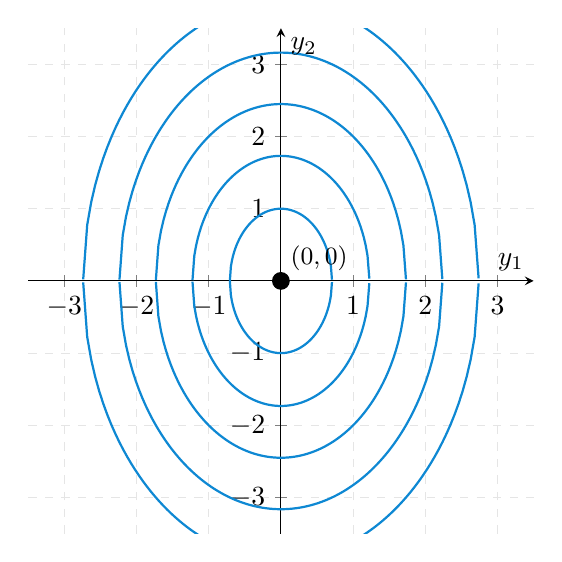
\begin{tikzpicture}
    \begin{axis}[
        xmin=-3.5, xmax=3.5,
        ymin=-3.5, ymax=3.5,
        axis lines=middle,
        xlabel={$y_1$},
        ylabel={$y_2$},
        samples=50,
        domain=-3.5:3.5,
        width=8cm,
        height=8cm,
        grid=both,
        grid style={dashed, gray!20}
    ]

        % Órbitas elípticas
        \foreach \C in {1, 3, 6, 10, 15} {
            \addplot[domain=-sqrt(\C/2):sqrt(\C/2), samples=100, cyan!70!blue, thick] ({x}, {sqrt(\C - 2*(x^2))});
            \addplot[domain=-sqrt(\C/2):sqrt(\C/2), samples=100, cyan!70!blue, thick] ({x}, {-sqrt(\C - 2*(x^2))});
        }

        % Punto fijo en (0,0)
        \addplot[only marks, mark=*, mark size=3pt, black] coordinates {(0,0)};
        \node[above right, font=\small] at (axis cs:0,0) {$(0,0)$};

    \end{axis}
\end{tikzpicture}
\end{center}
\end{sol}
\begin{ejer}[6]
Utilizando Mathematica dibuje el mapa de fases de $y^{\prime\prime}+2 y=0$ (1.5 puntos) 
\end{ejer}
\begin{sol} Se presentan a continuación las resoluciones computacionales en Mathematica utilizando tres metodologías distintas para el sistema equivalente $y_1' = y_2$, $y_2' = -2y_1$.
\begin{enumerate}[a)]
    \item Método Analítico Exacto (DSolve)

\begin{lstlisting}[language=Mathematica] ClearAll["Global`*"]
sol = DSolve[{y1'[x] == y2[x], y2'[x] == -2 y1[x], y1[0] == 1, y2[0] == 0}, {y1, y2}, x];
y1Fun = y1 /. sol[[1]];
y2Fun = y2 /. sol[[1]];
ParametricPlot[{y1Fun[x], y2Fun[x]}, {x, 0, 25},PlotStyle -> Green,AxesLabel -> {"Posicion (y)", "Velocidad (y')"},PlotLabel -> "Mapa de Fases Analitico"] \end{lstlisting}

    \item Método Numérico de Euler (Orden 1)

\begin{lstlisting}[language=Mathematica] ClearAll["Global`*"]
f[t_, Y_] := {Y[[2]], -2 Y[[1]]};
ci = {{1.0, 0.0}, {2.0, 0.0}, {3.0, 0.0}};
lc = Length[ci];
t0 = 0;
tf = 25; 
h = 0.05;
pasos = IntegerPart[(tf - t0)/h] + 1;
mapasDeFasesEuler = Table[{}, {i, 1, lc}];
Do[tn = t0; 
    Yn = ci[[j]];
    AppendTo[mapasDeFasesEuler[[j]], Yn];
    Do[Yn = Yn + h * f[tn, Yn]; (* Iteracion de Euler Expl\'icito *)
        tn = tn + h;
        AppendTo[mapasDeFasesEuler[[j]], Yn];,
        {i, 1, pasos}];
    , {j, 1, lc}]
ListLinePlot[mapasDeFasesEuler,AxesLabel -> {"Posicion", "Velocidad"},PlotLabel -> "Mapa de Fases Num\'erico (Euler)",PlotStyle -> Thick]\end{lstlisting} 

\item Método Numérico Punto Medio RK2 (Ejercicio 5)

\begin{lstlisting}[language=Mathematica] ClearAll["Global`*"]
f[t_, Y_] := {Y[[2]], -2 Y[[1]]};
ci = {{1.0, 0.0}, {2.0, 0.0}, {3.0, 0.0}};
lc = Length[ci];
t0 = 0; 
tf = 25; 
h = 0.05; 
h2 = h/2;
pasos = IntegerPart[(tf - t0)/h] + 1;
mapasDeFasesRK2 = Table[{}, {i, 1, lc}];
Do[tn = t0; 
    Yn = ci[[j]];
    AppendTo[mapasDeFasesRK2[[j]], Yn];
        Do[k1 = f[tn, Yn];
        k2 = f[tn + h2, Yn + h2 * k1];
        Yn = Yn + h * k2;
        tn = tn + h;
        AppendTo[mapasDeFasesRK2[[j]], Yn];
        , {i, 1, pasos}];
    , {j, 1, lc}]
ListLinePlot[mapasDeFasesRK2,AxesLabel -> {"Posicion", "Velocidad"},PlotLabel -> "Mapa de Fases Num\'erico (RK2 Punto Medio)",PlotStyle -> Thick]\end{lstlisting}
\end{enumerate} 
\end{sol}
